% !TEX program = xelatex
% Options for packages loaded elsewhere
\PassOptionsToPackage{unicode}{hyperref}
\PassOptionsToPackage{hyphens}{url}
%
\documentclass[
  12pt
]{article}
\usepackage[margin=1in]{geometry}
\usepackage{amsmath,amssymb}
\usepackage{graphicx}
\usepackage{etoolbox}
\AtBeginEnvironment{tabular*}{\small\setlength{\tabcolsep}{3pt}}
\AtBeginEnvironment{longtable}{\small}
\usepackage{tikz}
\usetikzlibrary{arrows.meta,shapes.geometric}
\usepackage{lmodern}
\usepackage{iftex}
\ifPDFTeX
  \usepackage[T1]{fontenc}
  \usepackage[utf8]{inputenc}
  \usepackage{textcomp} % provide euro and other symbols
\else % if luatex or xetex
  \usepackage{unicode-math}
  \defaultfontfeatures{Scale=MatchLowercase}
  \defaultfontfeatures[\rmfamily]{Ligatures=TeX,Scale=1}
\fi
% Use upquote if available, for straight quotes in verbatim environments
\IfFileExists{upquote.sty}{\usepackage{upquote}}{}
\IfFileExists{microtype.sty}{% use microtype if available
  \usepackage[]{microtype}
  \UseMicrotypeSet[protrusion]{basicmath} % disable protrusion for tt fonts
}{}
\makeatletter
\@ifundefined{KOMAClassName}{% if non-KOMA class
  \IfFileExists{parskip.sty}{%
    \usepackage{parskip}
  }{% else
    \setlength{\parindent}{0pt}
    \setlength{\parskip}{6pt plus 2pt minus 1pt}}
}{% if KOMA class
  \KOMAoptions{parskip=half}}
\makeatother
\usepackage{xcolor}
\IfFileExists{xurl.sty}{\usepackage{xurl}}{} % add URL line breaks if available
\IfFileExists{bookmark.sty}{\usepackage{bookmark}}{\usepackage{hyperref}}
\hypersetup{
  hidelinks,
  pdfcreator={LaTeX via pandoc}}
\urlstyle{same} % disable monospaced font for URLs
\usepackage{longtable,booktabs,array}
\usepackage{calc}
\usepackage{needspace} % keep table captions with their tables
% Correct order of tables after \paragraph or \subparagraph
\usepackage{etoolbox}
\makeatletter
\patchcmd\longtable{\par}{\if@noskipsec\mbox{}\fi\par}{}{}
\makeatother
% Allow footnotes in longtable head/foot
\IfFileExists{footnotehyper.sty}{\usepackage{footnotehyper}}{\usepackage{footnote}}
\makesavenoteenv{longtable}
\setlength{\emergencystretch}{3em} % prevent overfull lines
\providecommand{\tightlist}{%
  \setlength{\itemsep}{0pt}\setlength{\parskip}{0pt}}
\setcounter{secnumdepth}{-\maxdimen} % remove section numbering
\ifLuaTeX
  \usepackage{selnolig}  % disable illegal ligatures
\fi

\author{}
\date{}

\begin{document}

\hypertarget{factor-validation-of-activities}{%
\subsection{Factor Validation of Activities}\label{factor-validation-of-activities}}

The sociology of taste focuses on how everyday practices coalesce into broader lifestyle configurations, whether organized along traditional hierarchies of highbrow exclusion, expansive configurations of omnivorous engagement, or functional divisions between public participation and domestic routine. We analyze past-year participation frequencies across 20 distinct activities spanning institutional highbrow arts, commercial entertainment, domestic tasks, and solitary leisure routines. Because responses are recorded on an ordinal seven-point frequency scale, we estimate principal components on the polychoric correlation matrix using varimax rotation to establish an initial exploratory assignment of items to cultural domains.\footnote{Polychoric correlations estimate the association between the continuous propensities that generate each pair of ordinal responses, not the correlations among the coarse observed categories, and are the appropriate input when items are measured on ordered scales with few categories.}  The three-component solution accounts for 63.2 percent of total variance, supported by a Kaiser-Meyer-Olkin sampling adequacy metric of .955 (Table 1).\footnote{Complete responses on all 20 items are available for 1,243 respondents, who form the analytic sample for all measurement models. The Kaiser-Meyer-Olkin sampling adequacy statistic tells us whether the correlations among items are strong enough, relative to the correlations each item shares with the others and not with any particular partner, for a small set of shared dimensions to be worth extracting. A value of .955 indicates that the 20 items are well suited to the exercise.} 

The orthogonal solution divides the items between public, institutionalized cultural practices and private, domestic routines. Fourteen items coalesce into an expansive public arts factor, uniting traditional fine arts (symphonies, art galleries, theatrical performances) with broadly attended public events (festivals, movies, sporting events). Institutional arts and public amusements do not split into exclusive highbrow and commercial tiers; they form a single continuum of outward-facing cultural engagement. Three items---taking walks, regular exercise or yoga, and literary reading---cluster into an independent solitary leisure dimension centered on bodily maintenance and private contemplation. Three remaining practices---gardening, home or automobile repair, and infrequent dining at fast-food restaurants---define a residual practical-domestic dimension anchored in routine household maintenance.\footnote{We also estimated an exploratory factor analysis with direct oblimin rotation on the same polychoric matrix (Table A1). The oblique model fits the 20 items adequately ($\chi^2(133) = 290.8$, $p < .001$, $\text{TLI} = .911$, $\text{RMSEA} = .080$ $[.076, .084]$). Under direct oblimin, the public arts factor remains intact, but the secondary dimensions lose coherence. Assigning items based on highest loadings shifts literary reading, gardening, and home repair onto the arts factor, isolating fast food as a single-item residual. Forcing that assignment into confirmatory models yields inadmissible solutions, in which one or more parameters take values that no valid covariance matrix can sustain; the resulting solutions show negative residual variances and latent correlations exceeding unity. Because the oblique factor correlations in the exploratory solution are small (.19 between arts and leisure, $-.15$ between arts and residual, and $-.01$ between leisure and residual), the orthogonal and oblique orientations differ minimally in practice, and nothing in the data privileges one rotation over the other.}

We evaluate the varimax assignment against more parsimonious alternatives using confirmatory factor analysis with diagonally weighted least squares (WLSMV estimation, N = 1,243; Table 2), which relaxes the varimax orthogonality assumption by allowing the factors to be correlated. The three-factor model outperforms more parsimonious alternatives. Forcing residual practical items onto the arts factor produces a significant decrement in fit (scaled $\Delta\chi^2(2) = 121.6$, $p < .001$), as does forcing them onto solitary leisure ($\Delta\chi^2(2) = 51.0$, $p < .001$). A single-factor model specifying a generalized omnivorousness dimension performs worst of all ($\Delta\chi^2(3) = 146.4$, $p < .001$), showing that the cultural activity items included in the survey do not collapse into an undifferentiated propensity to consume across all domains. Although the three-factor confirmatory model fits better than any rival ($\text{CFI} = .956$, $\text{RMSEA} = .095$, $\text{SRMR} = .061$),\footnote{The comparative fit index (CFI) compares the fitted model with a null model in which the items are unrelated, with values closer to unity indicating better fit and values of at least .95 conventionally read as good fit. The root mean square error of approximation (RMSEA) reports misfit per degree of freedom, and the standardized root mean square residual (SRMR) reports the average discrepancy between the observed and implied correlations, with values below .08 conventionally read as acceptable for both. The Tucker-Lewis index (TLI), reported for the oblimin model in Table A1, adjusts the relative fit comparison for model parsimony. These cutoffs are rules of thumb, not tests, and we read them jointly, not one at a time.} the elevated RMSEA reflects the restrictive requirement that each practice load onto only a single factor. Everyday cultural activities naturally cross domain boundaries in ways that strict zero-loading constraints penalize.

To relax this assumption, we estimate an exploratory structural equation model (ESEM) using target rotation. The target matrix is built from the varimax primary-loading assignment, so each item is assigned to its primary factor and targeted toward zero on the other two. Because target rotation pulls off-target loadings toward zero instead of fixing them, items retain small, substantively plausible cross-loadings. The ESEM achieves a good fit to the observed polychoric covariances ($\text{CFI} = .979$, $\text{RMSEA} = .074$ $[.070, .079]$, $\text{SRMR} = .035$), improving over the confirmatory baseline (scaled $\Delta\chi^2(34) = 746.7$, $p < .001$; Table 2).\footnote{We retain the varimax targets because they align with the theoretical design of the battery, and Table A1 reports the oblimin solution of the same battery.}  Latent factor correlations confirm that while these three domains are distinct, they are modestly interrelated; public arts correlates positively with solitary leisure ($r = .36$) and residual domestic practices ($r = .21$), while leisure and residual practices correlate only weakly ($r = .11$; Table 3). 

All fourteen public arts items maintain primary loadings between .47 and .97 (Table 3). Solitary leisure is anchored firmly by walking (.78) and physical exercise (.42), though exercise also displays a secondary affinity with public cultural engagement (.32). Literary reading functions as the peripheral anchor of this leisure factor across all specifications (.44 in Table 1, .21 in Table A1, and .19 in Table 3), a structural attenuation that reflects its ambiguous status between solitary restorative practice and legitimate cultural capital. Domestic tasks (gardening at .45, home or auto repair at .32) and fast food avoidance ($-.38$) define the residual factor, on which institutional excursions (museums at .24, historic sites at .23) and outdoor recreation (hiking at .21) also load modestly. The factors differ sharply in reliability, with model-implied omegas of .97 for public arts, .74 for solitary leisure, and .68 for the residual factor (Table 3).\footnote{Omega is a reliability coefficient; it reports the share of the variance in a set of items that the intended common factor explains, generalizing Cronbach's alpha by weighting each item by its model-based loading rather than assuming that all items contribute equally. Because we compute it directly from the fitted ESEM, it accounts for the secondary cross-loadings as well as the primary loadings, and it is the reliability of the factor as the structural models actually use it.} Participation in several highbrow practices is sparse at the highest frequency, with only two respondents reporting that level for symphonies and for dance performances, and five for carnivals. Collapsing the top two categories in a sensitivity analysis leaves every factor assignment unchanged and shifts the CFA fit only in the third decimal place (CFI = .955 against .956; RMSEA = .095 in both).


\Needspace{38\baselineskip}
Table 1. Varimax Loadings for the Activity Battery

\begin{longtable}[]{@{}
  >{\raggedright\arraybackslash}p{(\columnwidth - 8\tabcolsep) * \real{0.4200}}
  >{\raggedright\arraybackslash}p{(\columnwidth - 8\tabcolsep) * \real{0.1600}}
  >{\raggedright\arraybackslash}p{(\columnwidth - 8\tabcolsep) * \real{0.1400}}
  >{\raggedright\arraybackslash}p{(\columnwidth - 8\tabcolsep) * \real{0.1400}}
  >{\raggedright\arraybackslash}p{(\columnwidth - 8\tabcolsep) * \real{0.1400}}@{}}
\toprule
Item & Assigned target & Arts & Leisure & Residual \\
\midrule
Museum & Arts & \textbf{0.80} & 0.21 & 0.21 \\
Art gallery & Arts & \textbf{0.83} & 0.19 & 0.20 \\
Symphony, orchestra, or opera & Arts & \textbf{0.89} & 0.06 & 0.23 \\
Carnival, fair, or amusement park & Arts & \textbf{0.83} & 0.13 & 0.01 \\
Music concert or festival & Arts & \textbf{0.84} & 0.17 & 0.02 \\
Play or musical & Arts & \textbf{0.84} & 0.09 & 0.13 \\
Library & Arts & \textbf{0.49} & 0.39 & 0.15 \\
Fancy restaurant & Arts & \textbf{0.72} & 0.26 & \llap{$-$}0.15 \\
Dance performance & Arts & \textbf{0.89} & 0.00 & 0.15 \\
Movie theater & Arts & \textbf{0.74} & 0.23 & \llap{$-$}0.24 \\
Attend sports & Arts & \textbf{0.79} & 0.21 & \llap{$-$}0.07 \\
Hiking, camping, or boating & Arts & \textbf{0.52} & 0.37 & 0.32 \\
Historic site & Arts & \textbf{0.70} & 0.23 & 0.26 \\
Go to festival & Arts & \textbf{0.78} & 0.27 & 0.15 \\
Go for a walk & Leisure & \llap{$-$}0.14 & \textbf{0.87} & 0.07 \\
Exercise or yoga & Leisure & 0.35 & \textbf{0.60} & \llap{$-$}0.19 \\
Read a novel, poem, or play & Leisure & 0.27 & \textbf{0.44} & 0.18 \\
Gardening & Residual & 0.27 & 0.31 & \textbf{0.62} \\
Fast food & Residual & 0.21 & 0.22 & \textbf{\llap{$-$}0.66} \\
Home auto repair & Residual & 0.38 & 0.24 & \textbf{0.49} \\
\midrule
\endhead
\bottomrule
\end{longtable}

Note. Varimax-rotated component loadings from a principal components analysis (N = 1,243). Bold entries mark each item's assigned factor. The assigned target column reports the factor on which each item is assigned in the ESEM targets. The three components together explain 63.2 percent of the variance.

\Needspace{26\baselineskip}
Table 2. Confirmatory and Exploratory Structural Models of the Activity Battery

\begin{longtable}[]{@{}
  >{\raggedright\arraybackslash}p{(\columnwidth - 12\tabcolsep) * \real{0.3000}}
  >{\raggedright\arraybackslash}p{(\columnwidth - 12\tabcolsep) * \real{0.0600}}
  >{\raggedright\arraybackslash}p{(\columnwidth - 12\tabcolsep) * \real{0.1200}}
  >{\raggedright\arraybackslash}p{(\columnwidth - 12\tabcolsep) * \real{0.0800}}
  >{\raggedright\arraybackslash}p{(\columnwidth - 12\tabcolsep) * \real{0.1000}}
  >{\raggedright\arraybackslash}p{(\columnwidth - 12\tabcolsep) * \real{0.1000}}
  >{\raggedright\arraybackslash}p{(\columnwidth - 12\tabcolsep) * \real{0.2400}}@{}}
\toprule
Model & df & Scaled $\chi^2$ & CFI & RMSEA & SRMR & Scaled $\Delta\chi^2$ (df) vs.~three-factor CFA \\
\midrule
One-factor CFA & 170 & 2225.5 & 0.952 & 0.099 & 0.064 & 146.4 (3), p \textless{} .001 \\
Two-factor CFA, residual merged into arts & 169 & 2199.3 & 0.952 & 0.098 & 0.063 & 121.6 (2), p \textless{} .001 \\
Two-factor CFA, residual merged into leisure & 169 & 2120.8 & 0.954 & 0.096 & 0.062 & 51.0 (2), p \textless{} .001 \\
Three-factor CFA & 167 & 2051.2 & 0.956 & 0.095 & 0.061 & --- \\
ESEM, target rotation & 133 & 1045.1 & 0.979 & 0.074 & 0.035 & 746.7 (34), p \textless{} .001 \\
\midrule
\endhead
\bottomrule
\end{longtable}

Note. N = 1,243. WLSMV estimation. The three-factor CFA is nested within the ESEM's implied covariance class as the case with zero cross-loadings, so the ESEM row reports a scaled difference test against it. The ESEM degrees of freedom reflect its rotation constraints. Latent factor correlations in the three-factor CFA are 0.76 (arts and leisure), 0.68 (arts and residual), and 0.59 (leisure and residual). RMSEA 90\% confidence intervals are [{..095, ..102}] (one-factor), [{..095, ..102}] (residual into arts), [{..093, ..100}] (residual into leisure), [{..092, ..099}] (three-factor), and [{..070, ..079}] (ESEM). Scaled difference tests use the Satorra-Bentler scaled statistic with per-model scaling factors.

\Needspace{38\baselineskip}
Table 3. ESEM Loadings with Target Rotation

\begin{longtable}[]{@{}
  >{\raggedright\arraybackslash}p{(\columnwidth - 8\tabcolsep) * \real{0.4200}}
  >{\raggedright\arraybackslash}p{(\columnwidth - 8\tabcolsep) * \real{0.1600}}
  >{\raggedright\arraybackslash}p{(\columnwidth - 8\tabcolsep) * \real{0.1400}}
  >{\raggedright\arraybackslash}p{(\columnwidth - 8\tabcolsep) * \real{0.1400}}
  >{\raggedright\arraybackslash}p{(\columnwidth - 8\tabcolsep) * \real{0.1400}}@{}}
\toprule
Item & Target factor & Arts & Leisure & Residual \\
\midrule
Museum & Arts & \textbf{0.78} & 0.03 & 0.24 \\
Art gallery & Arts & \textbf{0.83} & \llap{$-$}0.02 & 0.20 \\
Symphony, orchestra, or opera & Arts & \textbf{0.95} & \llap{$-$}0.22 & 0.11 \\
Carnival, fair, or amusement park & Arts & \textbf{0.82} & 0.04 & \llap{$-$}0.11 \\
Music concert or festival & Arts & \textbf{0.86} & 0.02 & \llap{$-$}0.11 \\
Play or musical & Arts & \textbf{0.90} & \llap{$-$}0.16 & 0.02 \\
Library & Arts & \textbf{0.47} & 0.16 & 0.14 \\
Fancy restaurant & Arts & \textbf{0.71} & 0.15 & \llap{$-$}0.20 \\
Dance performance & Arts & \textbf{0.97} & \llap{$-$}0.25 & 0.01 \\
Movie theater & Arts & \textbf{0.75} & 0.11 & \llap{$-$}0.30 \\
Attend sports & Arts & \textbf{0.80} & 0.08 & \llap{$-$}0.21 \\
Hiking, camping, or boating & Arts & \textbf{0.48} & 0.23 & 0.21 \\
Historic site & Arts & \textbf{0.65} & 0.11 & 0.23 \\
Go to festival & Arts & \textbf{0.78} & 0.10 & 0.04 \\
Go for a walk & Leisure & \llap{$-$}0.22 & \textbf{0.78} & 0.12 \\
Exercise or yoga & Leisure & 0.32 & \textbf{0.42} & \llap{$-$}0.17 \\
Read a novel, poem, or play & Leisure & 0.27 & \textbf{0.19} & 0.16 \\
Gardening & Residual & 0.23 & 0.17 & \textbf{0.45} \\
Fast food & Residual & 0.20 & 0.14 & \textbf{\llap{$-$}0.38} \\
Home auto repair & Residual & 0.34 & 0.14 & \textbf{0.32} \\
\midrule
Model-implied omega &  & 0.97 & 0.74 & 0.68 \\
\midrule
\endhead
\bottomrule
\end{longtable}

Note. Standardized loadings from an ESEM with target rotation (WLSMV, N = 1,243). Bold entries mark each item's assigned factor. Factor correlations: arts and leisure 0.36, arts and residual 0.21, leisure and residual 0.11. The final row reports the model-implied omega of each factor.


\subsection{Factor Validation of Network Composition}\label{factor-validation-of-network-composition}

Personal networks operate simultaneously as channels of social capital and instruments of symbolic boundary-making, serving as bridges across social space and conduits for homophily. The position generator batteries assess these relational structures across sixteen social categories, measured separately for casual acquaintances (weak ties) and close confidants (strong ties).\footnote{Gender items (knowing men, knowing women) are excluded because they display marked structural ambiguity across both relational domains. In exploratory analyses, knowing women splits nearly equally between the liberal and conservative factors in weak networks (.59 and .60), while knowing men loads heavily on both factors in weak ties (.68 and .57) and on conservative composition in strong ties (.62, alongside a .58 loading on liberal composition). In confirmatory models, retaining them lowers fit to $\text{CFI} = .896$ and $\text{RMSEA} = .116$ for weak ties and $\text{CFI} = .918$ and $\text{RMSEA} = .105$ for strong ties. Re-estimating regression models without the four gender items leaves every substantive finding and significance verdict intact, with no network coefficient shifting by more than .049.} Instead of an omnibus index of network diversity, the exploratory solutions identify three distinct relational structures in both spheres. The first captures a generalized breadth of ties spanning ethnic, geographic, and socioeconomic boundaries (Network Variety), while the second and third delineate distinct channels of partisan homophily (Liberal Composition and Conservative Composition). Demographic bridging and ideological sorting thus emerge as distinct relational dynamics; maintaining connections across varied social strata does not imply alignment with a particular political camp.

We put both the strong and weak tie batteries through the same analytic sequence as the activity items, from an exploratory decomposition to confirmatory testing to a target-rotated model. Principal components analysis of each battery's polychoric correlation matrix with varimax rotation gives us the initial assignment of each social position to variety, liberal composition, or conservative composition.\footnote{The varimax solutions show sampling adequacy of .939 for the weak-tie battery and .935 for the strong-tie battery, and each accounts for about 68 percent of the common variance; values this high, on the scale defined above, indicate that both batteries are well suited to the exercise.} Confirmatory factor models evaluating this three-factor structure show that strict simple-structure assumptions mischaracterize everyday network topology (Table A2), due to the fact that they penalize the natural secondary affinities among demographic and political identities forcing shared social space into the latent factor correlations.\footnote{In simple-structure confirmatory models, in which each item loads on a single factor and all other loadings are fixed at zero, freeing residual covariances between polar opposites (very liberal with very conservative, little church with lots of church, and city with rural) modestly improves fit (Table A2). Under the target-rotated ESEM, however, secondary cross-loadings absorb this bipolarity, rendering those residual covariances redundant and producing numerical instability in strong-tie estimation. We therefore retain the target ESEM without residual covariances.} In the CFA models without cross-factor loadings, the correlation between the network variety and the liberal composition factors rises to .81 in weak tie networks and .76 in strong tie networks, high enough to destabilize regression estimate due to collinearity. 

Target rotation helps alleviate the problem (Table 4), by letting positions display modest, substantively meaningful secondary affinities across the variety and composition factors for strong and weak ties. The ESEMs fit the data well in both batteries ($\text{CFI} = .979$, $\text{RMSEA} = .061$, $\text{SRMR} = .029$ for weak ties; $\text{CFI} = .975$, $\text{RMSEA} = .069$, $\text{SRMR} = .033$ for strong ties), showing that while demographic diversity and progressive sorting intersect in everyday networks, they remain distinct, moderately related dimensions, correlating .52 (variety and liberal composition), .45 (variety and conservative composition), and .47 (liberal and conservative composition) in weak ties, and .48, .54, and .34 in the same order in strong ties. All three network dimensions achieve high internal reliability across both tie types, with model-implied omegas between .90 and .93 for weak ties and between .88 and .94 for strong ties (Table 4). In the structural models that follow, both the network and activity blocks are the target-rotated ESEMs, with their loadings fixed at the target values, and the confirmatory factors serve as a comparison (Table A2).\footnote{We do not estimate a joint model that links the weak and strong factors in the main analysis. Without residual covariances between matching items, the joint model does not converge, and with them it converges only at a weakly identified solution, meaning one whose parameters the data leave imprecisely determined, in which the weak and strong variety factors correlate at .84 and the implied correlation of their disturbances, the unexplained shares of each factor, exceeds 1, an inadmissible value, while their leisure paths cancel. The separate models are therefore the basis for inference in both tie types.}

As Table 4 shows,factor loadings behave differently for racial diversity and political sorting at the two levels of tie strength. In casual acquaintance networks, minoritized racial and ethnic ties (Black and Hispanic acquaintances) straddle both network variety and progressive political composition. The dual affinity follows from the institutional organization of everyday social life. For many Americans, casual contact across racial lines occurs within progressive urban, educational, or professional environments. In close personal networks, by contrast, confidant ties to Black and Hispanic individuals anchor structural variety almost exclusively. When Americans form close, confiding bonds across racial lines, those ties represent genuine cross-boundary social bridging rather than incidental proximity to progressive politics. Conservative composition is the mirror image. Its relational boundary is tight in both weak and strong ties, anchored entirely by people who attend church, are conservative, live in rural areas, and identify as white. Ties to white people also display secondary affinities with liberal networks, capturing the partisan divide within the majority population, whereas conservative homophily remains structurally insular and segregated from ethnic diversity.


\Needspace{30\baselineskip}
Table 4. Standardized Loadings from the Target-Rotated ESEM of the Weak-Tie and Strong-Tie Batteries

\begin{tabular*}{\textwidth}{@{\extracolsep{\fill}}>{\raggedright\arraybackslash}p{0.30\textwidth} >{\raggedleft\arraybackslash}p{0.10\textwidth} >{\raggedleft\arraybackslash}p{0.10\textwidth} >{\raggedleft\arraybackslash}p{0.10\textwidth} >{\raggedleft\arraybackslash}p{0.10\textwidth} >{\raggedleft\arraybackslash}p{0.10\textwidth} >{\raggedleft\arraybackslash}p{0.10\textwidth}@{}}
\toprule
 & \multicolumn{3}{c}{Weak ties} & \multicolumn{3}{c}{Strong ties} \\
\cmidrule(lr){2-4}\cmidrule(lr){5-7}
Item & Variety & Lib. & Con. & Variety & Lib. & Con. \\
\midrule
Asian people & \textbf{\hphantom{$-$}0.61} & \hphantom{$-$}0.33 & $-$0.03 & \textbf{\hphantom{$-$}0.73} & \hphantom{$-$}0.15 & $-$0.06 \\
Second home & \textbf{\hphantom{$-$}0.50} & $-$0.03 & \hphantom{$-$}0.34 & \textbf{\hphantom{$-$}0.56} & $-$0.09 & \hphantom{$-$}0.31 \\
Born elsewhere & \textbf{\hphantom{$-$}0.48} & \hphantom{$-$}0.38 & \hphantom{$-$}0.02 & \textbf{\hphantom{$-$}0.70} & \hphantom{$-$}0.19 & $-$0.04 \\
MENA people & \textbf{\hphantom{$-$}0.77} & \hphantom{$-$}0.15 & \hphantom{$-$}0.00 & \textbf{\hphantom{$-$}0.88} & \hphantom{$-$}0.02 & $-$0.02 \\
NHPI people & \textbf{\hphantom{$-$}0.93} & $-$0.04 & $-$0.06 & \textbf{\hphantom{$-$}0.93} & $-$0.08 & $-$0.05 \\
American Indian people & \textbf{\hphantom{$-$}0.84} & $-$0.12 & \hphantom{$-$}0.06 & \textbf{\hphantom{$-$}0.85} & $-$0.14 & \hphantom{$-$}0.09 \\
LGBTQ people & \hphantom{$-$}0.03 & \textbf{\hphantom{$-$}0.80} & $-$0.07 & \hphantom{$-$}0.24 & \textbf{\hphantom{$-$}0.65} & $-$0.10 \\
Little church & $-$0.11 & \textbf{\hphantom{$-$}0.58} & \hphantom{$-$}0.32 & $-$0.07 & \textbf{\hphantom{$-$}0.54} & \hphantom{$-$}0.36 \\
Very liberal & $-$0.02 & \textbf{\hphantom{$-$}0.78} & \hphantom{$-$}0.05 & \hphantom{$-$}0.08 & \textbf{\hphantom{$-$}0.81} & $-$0.01 \\
Hispanic people & \hphantom{$-$}0.32 & \textbf{\hphantom{$-$}0.54} & \hphantom{$-$}0.01 & \textbf{\hphantom{$-$}0.59} & \hphantom{$-$}0.27 & $-$0.04 \\
Black people & \hphantom{$-$}0.36 & \textbf{\hphantom{$-$}0.36} & \hphantom{$-$}0.16 & \textbf{\hphantom{$-$}0.55} & \hphantom{$-$}0.18 & \hphantom{$-$}0.15 \\
City people & \hphantom{$-$}0.30 & \textbf{\hphantom{$-$}0.44} & \hphantom{$-$}0.07 & \hphantom{$-$}0.35 & \textbf{\hphantom{$-$}0.36} & \hphantom{$-$}0.12 \\
Lots of church & \hphantom{$-$}0.22 & $-$0.02 & \textbf{\hphantom{$-$}0.67} & \hphantom{$-$}0.29 & $-$0.09 & \textbf{\hphantom{$-$}0.63} \\
Very conservative & \hphantom{$-$}0.11 & $-$0.20 & \textbf{\hphantom{$-$}0.90} & \hphantom{$-$}0.14 & $-$0.20 & \textbf{\hphantom{$-$}0.81} \\
White people & $-$0.19 & \hphantom{$-$}0.41 & \textbf{\hphantom{$-$}0.68} & $-$0.15 & \hphantom{$-$}0.36 & \textbf{\hphantom{$-$}0.72} \\
Rural people & $-$0.07 & \hphantom{$-$}0.11 & \textbf{\hphantom{$-$}0.61} & $-$0.05 & \hphantom{$-$}0.16 & \textbf{\hphantom{$-$}0.60} \\
\midrule
Model-implied omega & 0.93 & 0.91 & 0.90 & 0.94 & 0.88 & 0.88 \\
\bottomrule
\end{tabular*}

Note. Standardized loadings from exploratory structural equation models with target rotation (WLSMV, polychoric; N = 1,258 per battery). Bold entries are the primary loadings from the target, and all other loadings are estimated rather than fixed at zero. Gender items are excluded. Factor correlations are 0.52 (variety and liberal), 0.45 (variety and conservative), and 0.47 (liberal and conservative) for weak ties, and 0.48, 0.54, and 0.34 in the same order for strong ties. Item labels are abbreviated from the variable names; MENA is Middle Eastern or North African, and NHPI is Native Hawaiian or Pacific Islander. Lib. and Con. denote liberal and conservative composition. The final row reports the model-implied omega of each factor.


\subsection{Structural Models of Activity Participation}\label{structural-models-of-activity-participation}

We estimate one structural equation model for each tie type rather than a single model for both, because estimating the two together produces parameter values that no valid covariance model can sustain. Each model regresses the three activity factors (public arts, solitary leisure, and practical-domestic residual activity) on the three network factors (variety, liberal composition, and conservative composition), and both blocks keep the measurement model established in the previous section, the target-rotated ESEM that retains secondary loadings instead of forcing them to zero. That choice is deliberate. Polar-opposite items, such as knowing very liberal and knowing very conservative people, load not only on their assigned factor but also, more weakly, on the opposing one. Confirmatory models that set these secondary connections to zero fit the data poorly, or else need patchwork residual correlations between the opposite items that the retained secondary loadings make unnecessary (Table A2).

The structural models keep the loadings, including the small secondary ones, at the values estimated in the measurement step and do not estimate them again inside the structural model. The reason to fix them is that estimating the loadings, the covariate regressions, and the network-to-activity paths all at once makes the models unstable, and covariate coefficients then come out with signs that contradict the item-level associations; fixing the loadings removes that instability and ties the structural paths to the validated solution in the measurement models reported earlier. Fixed loadings also keep the uncertainty in the loadings from leaking into the standard errors of the structural paths.\footnote{The factor correlations implied by the fixed loadings depend on the rotation chosen, and a split-half comparison with an oblimin rotation is reported in Table A3. Because these survey data are cross-sectional, the paths describe patterns of relational association rather than causal order. The residual factor has marginal reliability ($\omega = .68$; Table 3), so its paths should be read cautiously.} The cost is some loss of fit, which comes from the added covariate and network-to-activity regressions rather than from fixing the loadings.\footnote{Re-estimating the measurement model with the loadings held at their target values, both blocks freely correlated, and no covariate or network-to-activity regressions yields $\text{CFI} = .988$, $\text{RMSEA} = .029$, and $\text{SRMR} = .043$ for weak ties and $\text{CFI} = .987$, $\text{RMSEA} = .030$, and $\text{SRMR} = .044$ for strong ties on the same complete-case sample. Because fixing the loadings changes the degrees of freedom, these indices are not strictly comparable with those of the free measurement models, and the comparison supports one conclusion, that fixing the loadings costs no meaningful fit, which leaves the added regressions as the source of the fit loss in the structural models.}

Every item in both blocks is ordinal, so both models are estimated by weighted least squares with mean and variance adjustment (WLSMV) on polychoric correlations. Gender, race and ethnicity, childhood arts exposure, household income, age in years, and political ideology (1 to 7) predict every network and activity factor. The covariates work as controls, keeping the network-to-activity paths from simply tracking the sociodemographic composition of respondents. They are also predictors in their own right, and we decompose their total effects into direct and network-mediated components in labeled versions of the same models, in which every path is named so that the products along mediated routes can be summed (Tables 9 and 10). Education enters as a single ordinal variable running from high school or less (1) to graduate credentials (4). Estimation uses complete cases (N = 1,227), and both models converge with positive definite latent covariance matrices. Fit is adequate but weaker than that of the measurement models estimated without covariates ($\text{CFI} = .891$, $\text{RMSEA} = .058$, $\text{SRMR} = .075$ for weak ties; $\text{CFI} = .862$, $\text{RMSEA} = .066$, $\text{SRMR} = .086$ for strong ties), a difference consistent with holding the cross-loadings at their target values while adding covariate regressions.

The results trace a chain from social position to network composition to practice. We begin with the sociodemographic and ideological sources of network diversity and political composition (Tables 6 and 7), then turn to how network variety and composition relate to participation across public and private cultural domains (Table 5). The decomposition of early socialization, education, and political ideology into direct cultural orientations and network-mediated pathways comes next (Tables 9 and 10, diagrammed in Figures 5 to 10), followed by the baseline sociodemographic effects on each activity domain (Table 8). Every coefficient along this chain is a direct path net of the other predictors, and the decomposition shows how those direct associations combine with mediated routes into total effects.

\subsubsection{Sociodemographic Gradients in Network Composition}\label{sociodemographic-gradients-in-network-composition}

The covariate estimates reproduce familiar sociodemographic gradients on social capital and network composition, and they show sharp ideological sorting (Tables 6 and 7). Education has a positive effect on network variety in both tie types (.26 for weak and strong ties), replicating the standard finding that socioeconomic status broadens network diversity and connects individuals across different social boundaries. Political ideology, by contrast, operates through intense homophily rather than structural expansiveness. The path from political conservatism to liberal composition is negative ($-.50$ weak, $-.54$ strong) while the path to conservative composition is positive (.39 weak, .43 strong), showing that personal networks in the contemporary United States are sharply divided along ideological lines. Among the demographic characteristics, race and ethnicity show the strongest paths to conservative composition, and those paths are negative for every non-White category. AAPI respondents show the largest negative effects on conservative composition ($-.20$ weak, $-.25$ strong), and Black, Hispanic, and multiracial respondents show comparable negative effects. Because ties to racial minorities co-load structurally with liberal contacts, these negative paths indicate that the personal networks of White respondents tilt toward conservative composition whereas the networks of non-White respondents tilt toward liberal composition. Racial homophily in personal networks and political sorting are closely linked in everyday social ties.

\subsubsection{Network Effects on Activity Participation}\label{network-effects-on-activity-participation}

Network variety, rather than composition, is the main relational channel for public arts attendance in both tie types. Variety has standardized paths of .19 for weak ties and .25 for strong ties (both $p < .001$; Table 5), while liberal and conservative composition each have small positive paths to arts, between .04 and .08, all significant at $p < .001$, so the variety path is roughly 4 times their size among weak ties and between 3 and 6 times their size among strong ties. The weak liberal path is the least settled of these coefficients.\footnote{Under an oblimin rotation of the same specification, estimated separately in random halves of the sample (seed 4217), the variety paths on arts stay positive in every half for both tie types, while the weak liberal path on arts is near zero and changes sign across halves. We therefore treat the liberal path on arts as unstable. The liberal paths on solitary leisure are positive under both rotations.} These estimates support the Network Variety Model for institutional cultural participation. Attending symphonies, art galleries, live theater, and cultural festivals demands social coordination, cultural information, and shared co-presence. Individuals with expansive networks across diverse occupational positions encounter frequent invitations, casual cultural recommendations, and normative validation for arts attendance. The larger strong-tie variety path (.25) shows that coordinating attendance at high-commitment cultural events depends heavily on close social companions. Public arts participation runs through structural network expansiveness, not ideological alignment.

Solitary leisure reverses the pattern. Weak liberal composition (.20) and strong liberal composition (.22) have positive effects, significant at $p < .001$, while network variety and conservative composition are null in both tie types (weak variety .06, $p = .19$; strong variety $-.05$, $p = .27$). Solitary leisure activities, such as walking, regular exercise or yoga, and literary reading, involve minimal coordination friction and require no social co-presence, so general network diversity provides no logistical push toward their enactment. Instead, wellness routines, physical fitness, and reading are culturally coded within contemporary liberal life, and liberal peers sustain them as expressive practices. Paths to practical-domestic residual activity are smaller and less consistent, with variety positive in both tie types (.10 for weak ties, $p = .009$; .11 for strong ties, $p = .006$) and weak liberal composition negative and marginal ($-.09$, $p = .06$). Practical tasks such as gardening and home repairs, together with infrequent fast-food dining, draw upon diverse instrumental ties for advice and practical support, while remaining largely disconnected from ideological lifestyle repertoires.

\subsubsection{Direct, Network-Mediated, and Total Effects of the Focal Predictors}\label{direct-network-mediated-and-total-effects-of-the-focal-predictors}

Education, childhood arts exposure, and political conservatism reach activity participation by two routes, one direct and one mediated by network composition. Tables 9 and 10 partition each total effect into the two, which separates the lasting imprint of early socialization and credentials from the relational structures adults construct. Education's total standardized effect on arts is .35 in both tie models, of which the network accounts for about 15 and 20 percent and the remaining 85 and 80 percent is direct, matching the direct paths of .30 and .28 (Table 8). Childhood arts exposure has a total effect of .27, of which about .05 (weak) and .07 (strong) runs through network composition, about 18 and 26 percent of the total, with the remaining 82 and 74 percent direct (.22 and .20). Education and childhood socialization thus foster adult arts attendance primarily by instilling durable cultural dispositions, but they also operate through a relational mechanism, expanding adult network diversity, which then facilitates arts engagement. The total effects are nearly identical across tie models, because the covariate-to-activity relations are unconstrained in both, so the tie comparison concerns how much of each total runs through the network.\footnote{The total effects differ by no more than .004 between the weak-tie and strong-tie models for every predictor and activity factor. Only the split between direct and network-mediated routes differs by tie type.}

The effect of political conservatism on solitary leisure provides the clearest evidence of how network mediation can operate independently of direct individual tastes. Conservatism shows no significant direct path to solitary leisure in Table 8, yet its total effect on leisure is $-.12$ in both models ($p = .001$). The entire association is network-mediated through liberal composition, amounting to $-.07$ for weak ties ($p = .09$) and $-.11$ for strong ties ($p = .02$), which represents about 60 and 90 percent of the total, with the strong-tie channel clearing conventional statistical thresholds. The indirect channel follows from the network gradients reported earlier, where political conservatism reduces ties to liberals. Because liberal ties serve as the primary relational conduit encouraging solitary leisure, ideological sorting away from liberal peers indirectly suppresses participation in everyday leisure. For public arts, conservatism has a modest total effect of .09, of which the network route accounts for about .02 in weak ties and about .04 in strong ties, about 24 and 41 percent of the total, with both mediated paths significant at $p < .01$; the direct path is about .07 for weak ties and about .05 for strong ties. Network-mediated effects are summed over the three network factors and assume that the covariates do not confound the network-to-activity paths.

\subsubsection{Other Sociodemographic Direct Effects on Activity Factors}\label{other-sociodemographic-direct-effects-on-activity-factors}

The remaining direct effects on the activity factors (Table 8) mark the baseline levels of cultural stratification in this sample. Household income has a small positive direct path to arts and a negative effect on solitary leisure in both tie models, reflecting the material resources required for ticketed cultural events and the economic pressures that constrain leisure time. Age shows a distinct life-course divergence, predicting engagement in practical-domestic routines positively and public arts attendance negatively, a pattern reflecting both physical mobility constraints and the accumulation of domestic responsibilities over the life course. Gender differences on arts and leisure are negligible net of networks and background controls, though men participate slightly less in practical-domestic routines. Black, Hispanic, and multiracial respondents show negative direct paths to practical-domestic activities, and AAPI respondents report lower arts participation in both tie models ($-.07$ weak, $-.06$ strong). The AAPI gap in arts participation persists even after adjusting for education, income, childhood arts exposure, and network variety, which suggests that institutional arts spaces may keep subtle barriers to inclusion that socioeconomic and network advantages do not remove.


\Needspace{14\baselineskip}
Table 5. Standardized Network-to-Activity Paths from the Separate Weak-Tie and Strong-Tie Structural Models

\begin{tabular*}{\textwidth}{@{\extracolsep{\fill}}>{\raggedright\arraybackslash}p{0.36\textwidth} @{\hspace{1pt}}>{\raggedleft\arraybackslash}p{0.193\textwidth}@{\hspace{1pt}}>{\raggedleft\arraybackslash}p{0.193\textwidth}@{\hspace{1pt}}>{\raggedleft\arraybackslash}p{0.193\textwidth}@{\hspace{1.5em}}@{}}
\toprule
Network factor & Arts & Solitary leisure & Residual \\
\midrule
Weak variety & \hphantom{$-$}0.19\rlap{***} & \hphantom{$-$}0.06 & \hphantom{$-$}0.10\rlap{**} \\
Weak liberal & \hphantom{$-$}0.05\rlap{***} & \hphantom{$-$}0.20\rlap{***} & $-$0.09 \\
Weak conservative & \hphantom{$-$}0.04\rlap{***} & \hphantom{$-$}0.05 & $-$0.01 \\
Strong variety & \hphantom{$-$}0.25\rlap{***} & $-$0.05 & \hphantom{$-$}0.11\rlap{**} \\
Strong liberal & \hphantom{$-$}0.04\rlap{***} & \hphantom{$-$}0.22\rlap{***} & $-$0.04 \\
Strong conservative & \hphantom{$-$}0.08\rlap{***} & \hphantom{$-$}0.03 & \hphantom{$-$}0.01 \\
\bottomrule
\end{tabular*}

Note. Standardized coefficients from separate WLSMV structural models for weak ties and strong ties (N = 1,227 each), with loadings fixed at the target rotation of each battery. Each model includes gender, education, childhood arts exposure, income, age, race and ethnicity, and political ideology as predictors of all factors. * p < .05, ** p < .01, *** p < .001.

\Needspace{20\baselineskip}
Table 6. Sociodemographic Predictors of Weak-Tie Network Factors

\begin{tabular*}{\textwidth}{@{\extracolsep{\fill}}>{\raggedright\arraybackslash}p{0.36\textwidth} @{\hspace{1pt}}>{\raggedleft\arraybackslash}p{0.193\textwidth}@{\hspace{1pt}}>{\raggedleft\arraybackslash}p{0.193\textwidth}@{\hspace{1pt}}>{\raggedleft\arraybackslash}p{0.193\textwidth}@{\hspace{1.5em}}@{}}
\toprule
Predictor & Variety & Liberal & Conservative \\
\midrule
Age (years) & $-$0.13\rlap{***} & \hphantom{$-$}0.02 & \hphantom{$-$}0.05 \\
Education (1 to 4) & \hphantom{$-$}0.26\rlap{***} & \hphantom{$-$}0.00 & \hphantom{$-$}0.07\rlap{*} \\
Childhood arts & \hphantom{$-$}0.25\rlap{***} & \hphantom{$-$}0.06\rlap{*} & \hphantom{$-$}0.00 \\
Household income & \hphantom{$-$}0.05 & \hphantom{$-$}0.05 & \hphantom{$-$}0.08\rlap{**} \\
Political ideology (1 to 7) & \hphantom{$-$}0.15\rlap{***} & $-$0.50\rlap{***} & \hphantom{$-$}0.39\rlap{***} \\
Man (ref. woman) & \hphantom{$-$}0.05 & $-$0.10\rlap{***} & $-$0.07\rlap{*} \\
Non-binary/trans & $-$0.05 & \hphantom{$-$}0.00 & $-$0.06\rlap{*} \\
Black (ref. White) & \hphantom{$-$}0.17\rlap{***} & $-$0.09\rlap{***} & $-$0.15\rlap{***} \\
Hispanic (ref. White) & \hphantom{$-$}0.10\rlap{***} & \hphantom{$-$}0.02 & $-$0.18\rlap{***} \\
AAPI (ref. White) & \hphantom{$-$}0.10\rlap{***} & \hphantom{$-$}0.01 & $-$0.20\rlap{***} \\
Mixed/other (ref. White) & \hphantom{$-$}0.10\rlap{***} & \hphantom{$-$}0.01 & $-$0.15\rlap{***} \\
\bottomrule
\end{tabular*}

Note. Standardized coefficients from the weak-tie structural model (N = 1,227). Reference categories are shown in parentheses, and woman is the gender reference category. Political ideology ranges from 1 (very liberal) to 7 (very conservative). * p < .05, ** p < .01, *** p < .001.

\Needspace{20\baselineskip}
Table 7. Sociodemographic Predictors of Strong-Tie Network Factors

\begin{tabular*}{\textwidth}{@{\extracolsep{\fill}}>{\raggedright\arraybackslash}p{0.36\textwidth} @{\hspace{1pt}}>{\raggedleft\arraybackslash}p{0.193\textwidth}@{\hspace{1pt}}>{\raggedleft\arraybackslash}p{0.193\textwidth}@{\hspace{1pt}}>{\raggedleft\arraybackslash}p{0.193\textwidth}@{\hspace{1.5em}}@{}}
\toprule
Predictor & Variety & Liberal & Conservative \\
\midrule
Age (years) & $-$0.14\rlap{***} & \hphantom{$-$}0.05 & \hphantom{$-$}0.07\rlap{**} \\
Education (1 to 4) & \hphantom{$-$}0.26\rlap{***} & $-$0.01 & \hphantom{$-$}0.06\rlap{*} \\
Childhood arts & \hphantom{$-$}0.27\rlap{***} & \hphantom{$-$}0.06\rlap{*} & \hphantom{$-$}0.00 \\
Household income & $-$0.01 & \hphantom{$-$}0.09\rlap{**} & \hphantom{$-$}0.02 \\
Political ideology (1 to 7) & \hphantom{$-$}0.11\rlap{***} & $-$0.54\rlap{***} & \hphantom{$-$}0.43\rlap{***} \\
Man (ref. woman) & \hphantom{$-$}0.01 & $-$0.09\rlap{**} & $-$0.07\rlap{*} \\
Non-binary/trans & $-$0.03 & \hphantom{$-$}0.01 & $-$0.04 \\
Black (ref. White) & \hphantom{$-$}0.18\rlap{***} & $-$0.13\rlap{***} & $-$0.18\rlap{***} \\
Hispanic (ref. White) & \hphantom{$-$}0.13\rlap{***} & $-$0.04 & $-$0.18\rlap{***} \\
AAPI (ref. White) & \hphantom{$-$}0.10\rlap{***} & $-$0.09\rlap{***} & $-$0.25\rlap{***} \\
Mixed/other (ref. White) & \hphantom{$-$}0.10\rlap{***} & $-$0.06\rlap{*} & $-$0.21\rlap{***} \\
\bottomrule
\end{tabular*}

Note. Standardized coefficients from the strong-tie structural model (N = 1,227). Reference categories are shown in parentheses, and woman is the gender reference category. Political ideology ranges from 1 (very liberal) to 7 (very conservative). * p < .05, ** p < .01, *** p < .001.

\Needspace{20\baselineskip}
Table 8. Sociodemographic Predictors of Weak- and Strong-Tie Activity Factors

\begin{tabular*}{\textwidth}{@{\extracolsep{\fill}}>{\raggedright\arraybackslash}p{0.27\textwidth}
@{\hspace{1pt}}>{\raggedleft\arraybackslash}p{0.112\textwidth}@{\hspace{1pt}}>{\raggedleft\arraybackslash}p{0.112\textwidth}@{\hspace{1pt}}>{\raggedleft\arraybackslash}p{0.112\textwidth}@{\hspace{1pt}}>{\raggedleft\arraybackslash}p{0.112\textwidth}@{\hspace{1pt}}>{\raggedleft\arraybackslash}p{0.112\textwidth}@{\hspace{1pt}}>{\raggedleft\arraybackslash}p{0.112\textwidth}@{}}
\toprule
 & \multicolumn{3}{c}{Weak ties} & \multicolumn{3}{c}{Strong ties} \\
\cmidrule(lr){2-4}\cmidrule(lr){5-7}
Predictor & Arts & Leisure & Residual & Arts & Leisure & Residual \\
\midrule
Age (years) & $-$0.13\rlap{***} & \hphantom{$-$}0.00 & \hphantom{$-$}0.38\rlap{***} & $-$0.13\rlap{***} & $-$0.02 & \hphantom{$-$}0.38\rlap{***} \\
Education (1 to 4) & \hphantom{$-$}0.30\rlap{***} & $-$0.01 & \hphantom{$-$}0.10\rlap{*} & \hphantom{$-$}0.28\rlap{***} & \hphantom{$-$}0.02 & \hphantom{$-$}0.10\rlap{*} \\
Childhood arts & \hphantom{$-$}0.22\rlap{***} & $-$0.07 & \hphantom{$-$}0.06 & \hphantom{$-$}0.20\rlap{***} & $-$0.04 & \hphantom{$-$}0.05 \\
Household income & \hphantom{$-$}0.06\rlap{**} & \hphantom{$-$}0.09\rlap{*} & $-$0.06 & \hphantom{$-$}0.07\rlap{**} & \hphantom{$-$}0.08\rlap{*} & $-$0.06 \\
Political ideology (1 to 7) & \hphantom{$-$}0.07\rlap{**} & $-$0.05 & $-$0.12\rlap{**} & \hphantom{$-$}0.05\rlap{*} & $-$0.01 & $-$0.11\rlap{*} \\
Man (ref. woman) & $-$0.01 & \hphantom{$-$}0.00 & $-$0.07\rlap{*} & \hphantom{$-$}0.00 & \hphantom{$-$}0.00 & $-$0.06 \\
Non-binary/trans & \hphantom{$-$}0.02 & $-$0.04 & \hphantom{$-$}0.06 & \hphantom{$-$}0.01 & $-$0.04 & \hphantom{$-$}0.06 \\
Black (ref. White) & \hphantom{$-$}0.04 & $-$0.07 & $-$0.21\rlap{***} & \hphantom{$-$}0.03 & $-$0.04 & $-$0.21\rlap{***} \\
Hispanic (ref. White) & \hphantom{$-$}0.01 & \hphantom{$-$}0.01 & $-$0.10\rlap{*} & \hphantom{$-$}0.01 & \hphantom{$-$}0.04 & $-$0.10\rlap{**} \\
AAPI (ref. White) & $-$0.07\rlap{**} & \hphantom{$-$}0.01 & \hphantom{$-$}0.00 & $-$0.06\rlap{**} & \hphantom{$-$}0.04 & \hphantom{$-$}0.00 \\
Mixed/other (ref. White) & $-$0.04 & \hphantom{$-$}0.04 & \hphantom{$-$}0.08\rlap{*} & $-$0.03 & \hphantom{$-$}0.06 & \hphantom{$-$}0.08\rlap{*} \\
\bottomrule
\end{tabular*}

Note. Standardized coefficients from the weak-tie and strong-tie structural models (N = 1,227 each). Reference categories are shown in parentheses, and woman is the gender reference category. Each activity equation also includes the three network factors of its tie type, whose coefficients are reported in Table 5. * p < .05, ** p < .01, *** p < .001.


\Needspace{18\baselineskip}
Figure 5. Paths from Education to Arts Participation, Weak Ties

\begin{center}
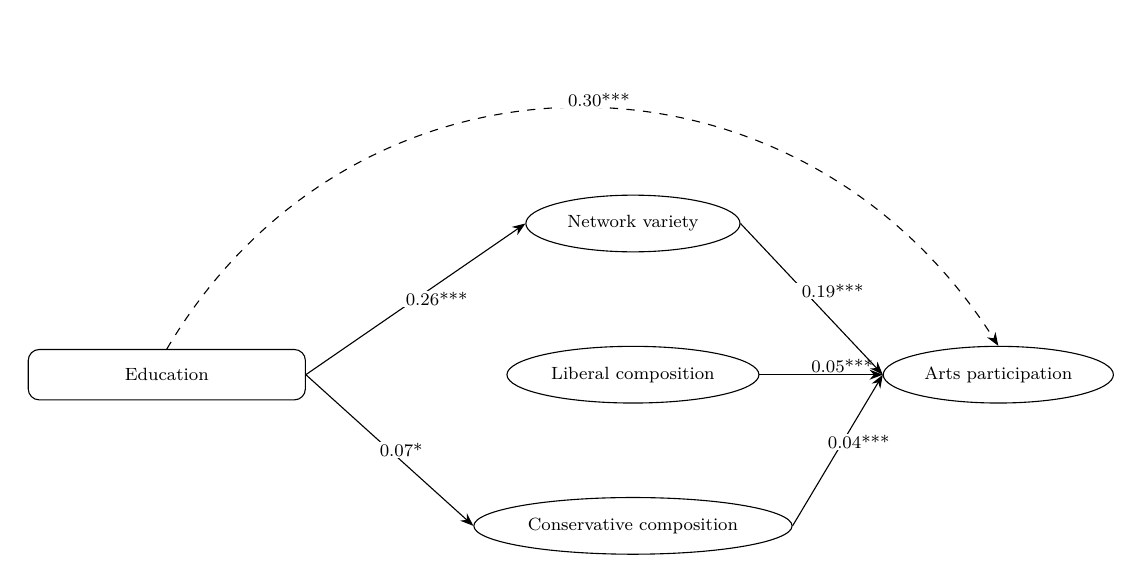
\begin{tikzpicture}[>=Stealth, font=\footnotesize, scale=0.8, transform shape,
  box/.style={draw, rounded corners, align=center, minimum width=4.4cm, minimum height=0.8cm},
  lat/.style={draw, ellipse, align=center, minimum width=3.4cm, minimum height=0.9cm},
  lab/.style={fill=white, inner sep=0.5pt, font=\footnotesize}]
\node[box] (x) at (0,0) {Education};
\node[lat] (wv) at (7.4,2.4) {Network variety};
\node[lat] (wl) at (7.4,0.0) {Liberal composition};
\node[lat] (wc) at (7.4,-2.4) {Conservative composition};
\node[lat] (act) at (13.2,0) {Arts participation};
\draw[->] (x.east) -- node[lab, pos=0.5] {\hphantom{$-$}0.26\rlap{***}} (wv.west);
\draw[->] (x.east) -- node[lab, pos=0.5] {\hphantom{$-$}0.07\rlap{*}} (wc.west);
\draw[->] (wv.east) -- node[lab, pos=0.5, above] {\hphantom{$-$}0.19\rlap{***}} (act.west);
\draw[->] (wl.east) -- node[lab, pos=0.5, above] {\hphantom{$-$}0.05\rlap{***}} (act.west);
\draw[->] (wc.east) -- node[lab, pos=0.5, above] {\hphantom{$-$}0.04\rlap{***}} (act.west);
\draw[->, dashed] (x.north) .. controls (3,5.5) and (10,5.5) .. node[lab, pos=0.5, above] {\hphantom{$-$}0.30\rlap{***}} (act.north);
\end{tikzpicture}
\end{center}

Note. Standardized coefficients from the weak-tie structural model with loadings fixed at the target rotation (N = 1,227). Solid arrows are paths through the network factors, dashed arrows are direct paths, and only paths significant at $p < .05$ are drawn. Asterisks follow Table 5.

\Needspace{18\baselineskip}
Figure 6. Paths from Childhood Arts Exposure to Arts Participation, Weak Ties

\begin{center}
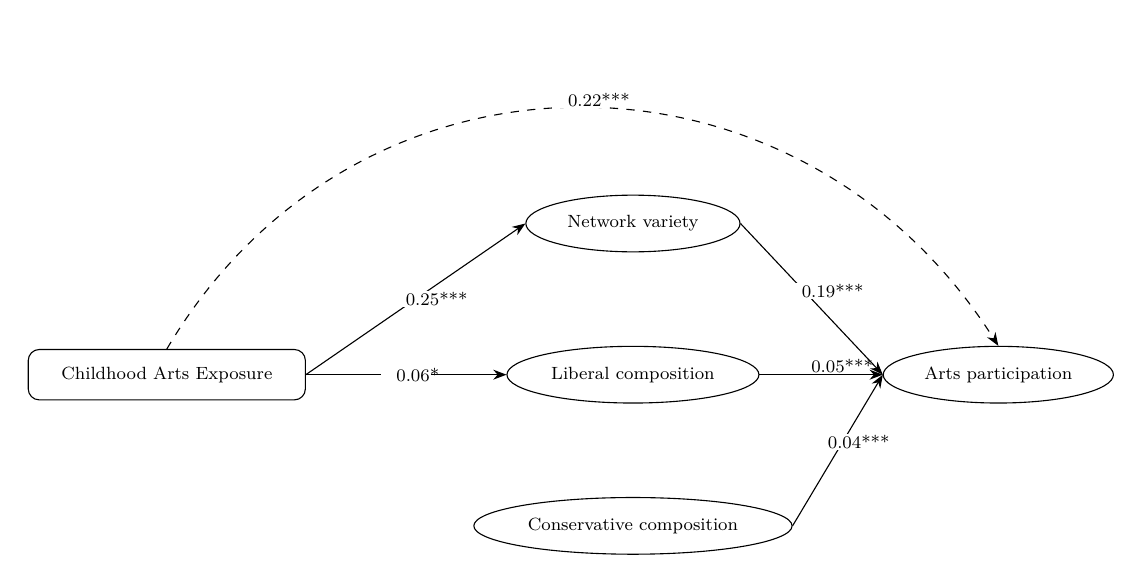
\begin{tikzpicture}[>=Stealth, font=\footnotesize, scale=0.8, transform shape,
  box/.style={draw, rounded corners, align=center, minimum width=4.4cm, minimum height=0.8cm},
  lat/.style={draw, ellipse, align=center, minimum width=3.4cm, minimum height=0.9cm},
  lab/.style={fill=white, inner sep=0.5pt, font=\footnotesize}]
\node[box] (x) at (0,0) {Childhood Arts Exposure};
\node[lat] (wv) at (7.4,2.4) {Network variety};
\node[lat] (wl) at (7.4,0.0) {Liberal composition};
\node[lat] (wc) at (7.4,-2.4) {Conservative composition};
\node[lat] (act) at (13.2,0) {Arts participation};
\draw[->] (x.east) -- node[lab, pos=0.5] {\hphantom{$-$}0.25\rlap{***}} (wv.west);
\draw[->] (x.east) -- node[lab, pos=0.5] {\hphantom{$-$}0.06\rlap{*}} (wl.west);
\draw[->] (wv.east) -- node[lab, pos=0.5, above] {\hphantom{$-$}0.19\rlap{***}} (act.west);
\draw[->] (wl.east) -- node[lab, pos=0.5, above] {\hphantom{$-$}0.05\rlap{***}} (act.west);
\draw[->] (wc.east) -- node[lab, pos=0.5, above] {\hphantom{$-$}0.04\rlap{***}} (act.west);
\draw[->, dashed] (x.north) .. controls (3,5.5) and (10,5.5) .. node[lab, pos=0.5, above] {\hphantom{$-$}0.22\rlap{***}} (act.north);
\end{tikzpicture}
\end{center}

Note. Standardized coefficients from the weak-tie structural model with loadings fixed at the target rotation (N = 1,227). Solid arrows are paths through the network factors, dashed arrows are direct paths, and only paths significant at $p < .05$ are drawn. Asterisks follow Table 5.

\Needspace{18\baselineskip}
Figure 7. Paths from Political Conservatism to Arts Participation, Weak Ties

\begin{center}
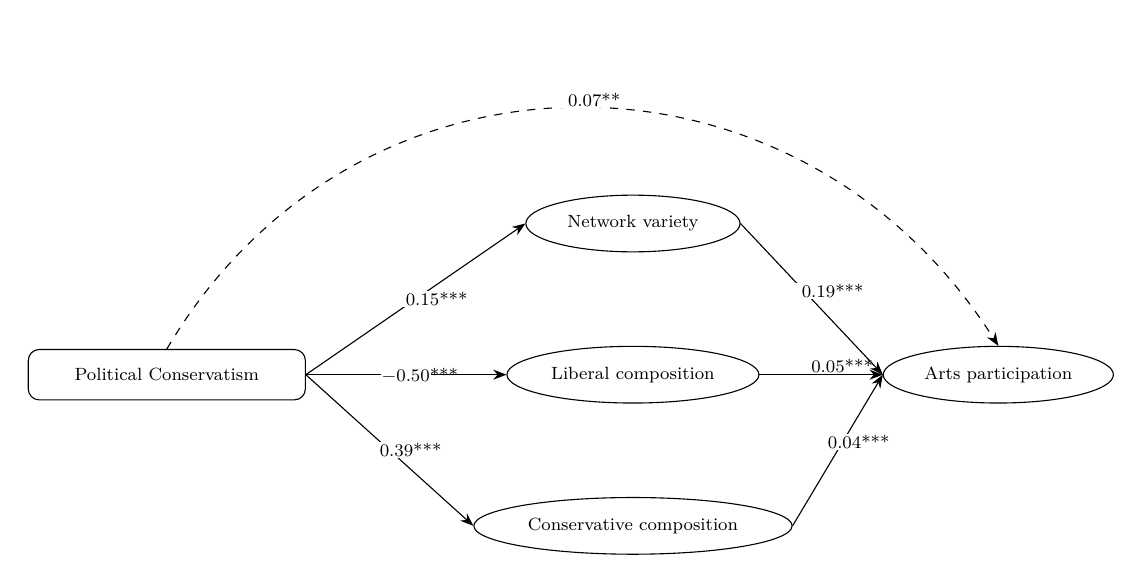
\begin{tikzpicture}[>=Stealth, font=\footnotesize, scale=0.8, transform shape,
  box/.style={draw, rounded corners, align=center, minimum width=4.4cm, minimum height=0.8cm},
  lat/.style={draw, ellipse, align=center, minimum width=3.4cm, minimum height=0.9cm},
  lab/.style={fill=white, inner sep=0.5pt, font=\footnotesize}]
\node[box] (x) at (0,0) {Political Conservatism};
\node[lat] (wv) at (7.4,2.4) {Network variety};
\node[lat] (wl) at (7.4,0.0) {Liberal composition};
\node[lat] (wc) at (7.4,-2.4) {Conservative composition};
\node[lat] (act) at (13.2,0) {Arts participation};
\draw[->] (x.east) -- node[lab, pos=0.5] {\hphantom{$-$}0.15\rlap{***}} (wv.west);
\draw[->] (x.east) -- node[lab, pos=0.5] {$-$0.50\rlap{***}} (wl.west);
\draw[->] (x.east) -- node[lab, pos=0.5] {\hphantom{$-$}0.39\rlap{***}} (wc.west);
\draw[->] (wv.east) -- node[lab, pos=0.5, above] {\hphantom{$-$}0.19\rlap{***}} (act.west);
\draw[->] (wl.east) -- node[lab, pos=0.5, above] {\hphantom{$-$}0.05\rlap{***}} (act.west);
\draw[->] (wc.east) -- node[lab, pos=0.5, above] {\hphantom{$-$}0.04\rlap{***}} (act.west);
\draw[->, dashed] (x.north) .. controls (3,5.5) and (10,5.5) .. node[lab, pos=0.5, above] {\hphantom{$-$}0.07\rlap{**}} (act.north);
\end{tikzpicture}
\end{center}

Note. Standardized coefficients from the weak-tie structural model with loadings fixed at the target rotation (N = 1,227). Solid arrows are paths through the network factors, dashed arrows are direct paths, and only paths significant at $p < .05$ are drawn. Asterisks follow Table 5.

\Needspace{18\baselineskip}
Figure 8. Paths from Education to Arts Participation, Strong Ties

\begin{center}
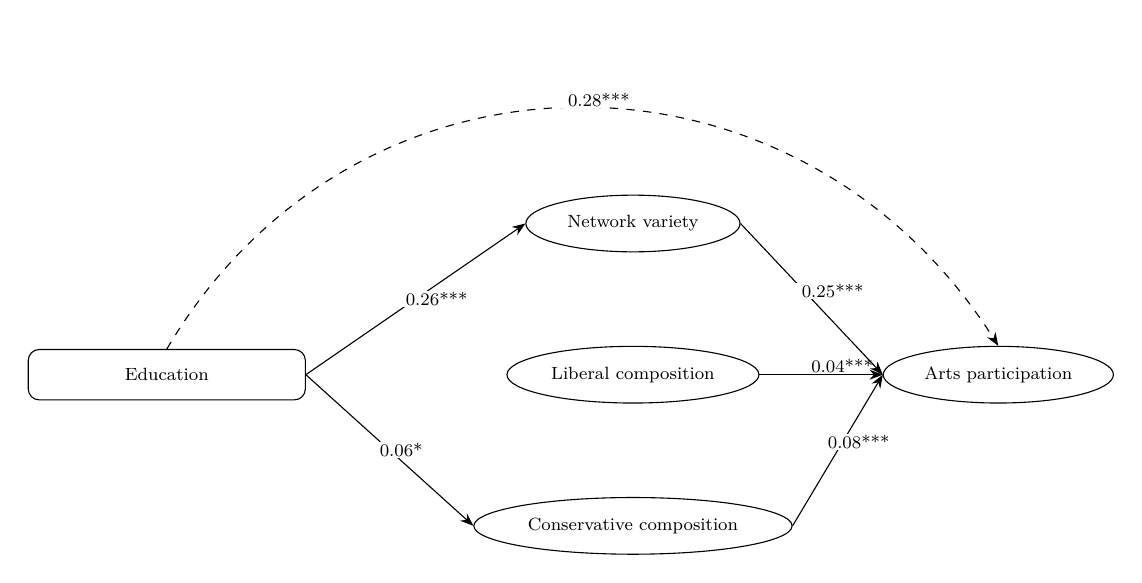
\begin{tikzpicture}[>=Stealth, font=\footnotesize, scale=0.8, transform shape,
  box/.style={draw, rounded corners, align=center, minimum width=4.4cm, minimum height=0.8cm},
  lat/.style={draw, ellipse, align=center, minimum width=3.4cm, minimum height=0.9cm},
  lab/.style={fill=white, inner sep=0.5pt, font=\footnotesize}]
\node[box] (x) at (0,0) {Education};
\node[lat] (wv) at (7.4,2.4) {Network variety};
\node[lat] (wl) at (7.4,0.0) {Liberal composition};
\node[lat] (wc) at (7.4,-2.4) {Conservative composition};
\node[lat] (act) at (13.2,0) {Arts participation};
\draw[->] (x.east) -- node[lab, pos=0.5] {\hphantom{$-$}0.26\rlap{***}} (wv.west);
\draw[->] (x.east) -- node[lab, pos=0.5] {\hphantom{$-$}0.06\rlap{*}} (wc.west);
\draw[->] (wv.east) -- node[lab, pos=0.5, above] {\hphantom{$-$}0.25\rlap{***}} (act.west);
\draw[->] (wl.east) -- node[lab, pos=0.5, above] {\hphantom{$-$}0.04\rlap{***}} (act.west);
\draw[->] (wc.east) -- node[lab, pos=0.5, above] {\hphantom{$-$}0.08\rlap{***}} (act.west);
\draw[->, dashed] (x.north) .. controls (3,5.5) and (10,5.5) .. node[lab, pos=0.5, above] {\hphantom{$-$}0.28\rlap{***}} (act.north);
\end{tikzpicture}
\end{center}

Note. Standardized coefficients from the strong-tie structural model with loadings fixed at the target rotation (N = 1,227). Solid arrows are paths through the network factors, dashed arrows are direct paths, and only paths significant at $p < .05$ are drawn. Asterisks follow Table 5.

\Needspace{18\baselineskip}
Figure 9. Paths from Childhood Arts Exposure to Arts Participation, Strong Ties

\begin{center}
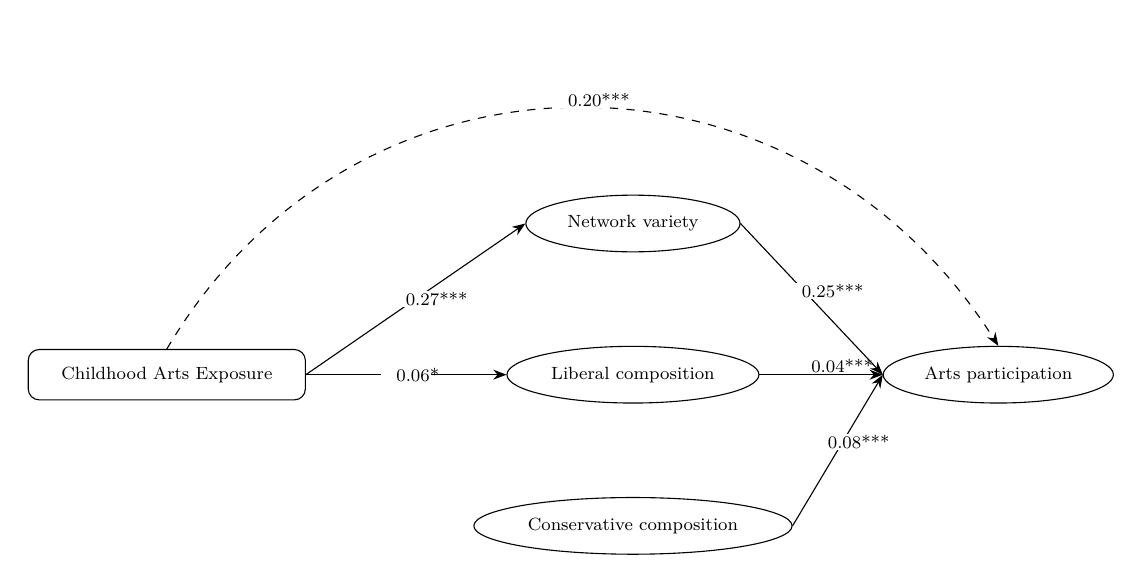
\begin{tikzpicture}[>=Stealth, font=\footnotesize, scale=0.8, transform shape,
  box/.style={draw, rounded corners, align=center, minimum width=4.4cm, minimum height=0.8cm},
  lat/.style={draw, ellipse, align=center, minimum width=3.4cm, minimum height=0.9cm},
  lab/.style={fill=white, inner sep=0.5pt, font=\footnotesize}]
\node[box] (x) at (0,0) {Childhood Arts Exposure};
\node[lat] (wv) at (7.4,2.4) {Network variety};
\node[lat] (wl) at (7.4,0.0) {Liberal composition};
\node[lat] (wc) at (7.4,-2.4) {Conservative composition};
\node[lat] (act) at (13.2,0) {Arts participation};
\draw[->] (x.east) -- node[lab, pos=0.5] {\hphantom{$-$}0.27\rlap{***}} (wv.west);
\draw[->] (x.east) -- node[lab, pos=0.5] {\hphantom{$-$}0.06\rlap{*}} (wl.west);
\draw[->] (wv.east) -- node[lab, pos=0.5, above] {\hphantom{$-$}0.25\rlap{***}} (act.west);
\draw[->] (wl.east) -- node[lab, pos=0.5, above] {\hphantom{$-$}0.04\rlap{***}} (act.west);
\draw[->] (wc.east) -- node[lab, pos=0.5, above] {\hphantom{$-$}0.08\rlap{***}} (act.west);
\draw[->, dashed] (x.north) .. controls (3,5.5) and (10,5.5) .. node[lab, pos=0.5, above] {\hphantom{$-$}0.20\rlap{***}} (act.north);
\end{tikzpicture}
\end{center}

Note. Standardized coefficients from the strong-tie structural model with loadings fixed at the target rotation (N = 1,227). Solid arrows are paths through the network factors, dashed arrows are direct paths, and only paths significant at $p < .05$ are drawn. Asterisks follow Table 5.

\Needspace{18\baselineskip}
Figure 10. Paths from Political Conservatism to Arts Participation, Strong Ties

\begin{center}
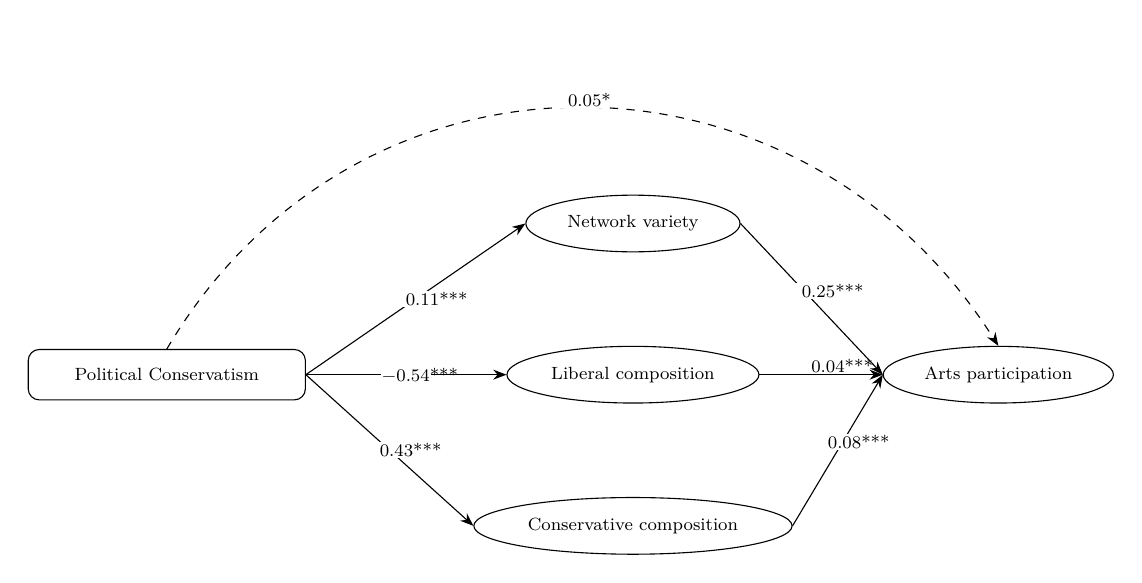
\begin{tikzpicture}[>=Stealth, font=\footnotesize, scale=0.8, transform shape,
  box/.style={draw, rounded corners, align=center, minimum width=4.4cm, minimum height=0.8cm},
  lat/.style={draw, ellipse, align=center, minimum width=3.4cm, minimum height=0.9cm},
  lab/.style={fill=white, inner sep=0.5pt, font=\footnotesize}]
\node[box] (x) at (0,0) {Political Conservatism};
\node[lat] (wv) at (7.4,2.4) {Network variety};
\node[lat] (wl) at (7.4,0.0) {Liberal composition};
\node[lat] (wc) at (7.4,-2.4) {Conservative composition};
\node[lat] (act) at (13.2,0) {Arts participation};
\draw[->] (x.east) -- node[lab, pos=0.5] {\hphantom{$-$}0.11\rlap{***}} (wv.west);
\draw[->] (x.east) -- node[lab, pos=0.5] {$-$0.54\rlap{***}} (wl.west);
\draw[->] (x.east) -- node[lab, pos=0.5] {\hphantom{$-$}0.43\rlap{***}} (wc.west);
\draw[->] (wv.east) -- node[lab, pos=0.5, above] {\hphantom{$-$}0.25\rlap{***}} (act.west);
\draw[->] (wl.east) -- node[lab, pos=0.5, above] {\hphantom{$-$}0.04\rlap{***}} (act.west);
\draw[->] (wc.east) -- node[lab, pos=0.5, above] {\hphantom{$-$}0.08\rlap{***}} (act.west);
\draw[->, dashed] (x.north) .. controls (3,5.5) and (10,5.5) .. node[lab, pos=0.5, above] {\hphantom{$-$}0.05\rlap{*}} (act.north);
\end{tikzpicture}
\end{center}

Note. Standardized coefficients from the strong-tie structural model with loadings fixed at the target rotation (N = 1,227). Solid arrows are paths through the network factors, dashed arrows are direct paths, and only paths significant at $p < .05$ are drawn. Asterisks follow Table 5.


\Needspace{18\baselineskip}
Table 9. Direct, Network-Mediated, and Total Standardized Effects of Education, Childhood Arts Exposure, and Political Ideology on the Activity Factors, Weak Ties

\begin{tabular*}{\textwidth}{@{\extracolsep{\fill}}>{\raggedright\arraybackslash}p{0.36\textwidth} @{\hspace{1pt}}>{\raggedleft\arraybackslash}p{0.193\textwidth}@{\hspace{1pt}}>{\raggedleft\arraybackslash}p{0.193\textwidth}@{\hspace{1pt}}>{\raggedleft\arraybackslash}p{0.193\textwidth}@{\hspace{1.5em}}@{}}
\toprule
Predictor and activity factor & Direct & Network-mediated & Total \\
\midrule
Arts: education & \hphantom{$-$}0.30\rlap{***} & \hphantom{$-$}0.05\rlap{***} & \hphantom{$-$}0.35\rlap{***} \\
Arts: childhood arts & \hphantom{$-$}0.22\rlap{***} & \hphantom{$-$}0.05\rlap{***} & \hphantom{$-$}0.27\rlap{***} \\
Arts: political ideology & \hphantom{$-$}0.07\rlap{**} & \hphantom{$-$}0.02\rlap{**} & \hphantom{$-$}0.09\rlap{***} \\
Leisure: education & $-$0.01 & \hphantom{$-$}0.02 & \hphantom{$-$}0.01 \\
Leisure: childhood arts & $-$0.07 & \hphantom{$-$}0.03\rlap{*} & $-$0.04 \\
Leisure: political ideology & $-$0.05 & $-$0.07 & $-$0.12\rlap{***} \\
Residual: education & \hphantom{$-$}0.10\rlap{*} & \hphantom{$-$}0.03\rlap{*} & \hphantom{$-$}0.13\rlap{**} \\
Residual: childhood arts & \hphantom{$-$}0.06 & \hphantom{$-$}0.02 & \hphantom{$-$}0.08\rlap{*} \\
Residual: political ideology & $-$0.12\rlap{**} & \hphantom{$-$}0.06 & $-$0.07\rlap{*} \\
\bottomrule
\end{tabular*}

Note. Standardized effects from the labeled weak-tie model. Network-mediated effects sum the products of each predictor's path to a network factor and that factor's path to the activity factor, with standard errors from the delta method, a first-order approximation that propagates the uncertainty of the component paths into each product. Total effects equal direct plus network-mediated effects. * p < .05, ** p < .01, *** p < .001.

\Needspace{18\baselineskip}
Table 10. Direct, Network-Mediated, and Total Standardized Effects of Education, Childhood Arts Exposure, and Political Ideology on the Activity Factors, Strong Ties

\begin{tabular*}{\textwidth}{@{\extracolsep{\fill}}>{\raggedright\arraybackslash}p{0.36\textwidth} @{\hspace{1pt}}>{\raggedleft\arraybackslash}p{0.193\textwidth}@{\hspace{1pt}}>{\raggedleft\arraybackslash}p{0.193\textwidth}@{\hspace{1pt}}>{\raggedleft\arraybackslash}p{0.193\textwidth}@{\hspace{1.5em}}@{}}
\toprule
Predictor and activity factor & Direct & Network-mediated & Total \\
\midrule
Arts: education & \hphantom{$-$}0.28\rlap{***} & \hphantom{$-$}0.07\rlap{***} & \hphantom{$-$}0.35\rlap{***} \\
Arts: childhood arts & \hphantom{$-$}0.20\rlap{***} & \hphantom{$-$}0.07\rlap{***} & \hphantom{$-$}0.27\rlap{***} \\
Arts: political ideology & \hphantom{$-$}0.05\rlap{*} & \hphantom{$-$}0.04\rlap{***} & \hphantom{$-$}0.09\rlap{***} \\
Leisure: education & \hphantom{$-$}0.02 & $-$0.01 & \hphantom{$-$}0.01 \\
Leisure: childhood arts & $-$0.04 & \hphantom{$-$}0.00 & $-$0.04 \\
Leisure: political ideology & $-$0.01 & $-$0.11\rlap{*} & $-$0.12\rlap{***} \\
Residual: education & \hphantom{$-$}0.10\rlap{*} & \hphantom{$-$}0.03\rlap{**} & \hphantom{$-$}0.13\rlap{**} \\
Residual: childhood arts & \hphantom{$-$}0.05 & \hphantom{$-$}0.03\rlap{*} & \hphantom{$-$}0.08\rlap{*} \\
Residual: political ideology & $-$0.11\rlap{*} & \hphantom{$-$}0.04 & $-$0.07\rlap{*} \\
\bottomrule
\end{tabular*}

Note. Standardized effects from the labeled strong-tie model. Network-mediated effects sum the products of each predictor's path to a network factor and that factor's path to the activity factor, with standard errors from the delta method, a first-order approximation that propagates the uncertainty of the component paths into each product. Total effects equal direct plus network-mediated effects. * p < .05, ** p < .01, *** p < .001.
\subsection*{Appendix: Supplementary Measurement and Robustness Models}

\Needspace{38\baselineskip}
Table A1. Oblimin-Rotated Exploratory Factor Loadings for the Activity Battery

\begin{longtable}[]{@{}
  >{\raggedright\arraybackslash}p{(\columnwidth - 8\tabcolsep) * \real{0.4200}}
  >{\raggedright\arraybackslash}p{(\columnwidth - 8\tabcolsep) * \real{0.1600}}
  >{\raggedright\arraybackslash}p{(\columnwidth - 8\tabcolsep) * \real{0.1400}}
  >{\raggedright\arraybackslash}p{(\columnwidth - 8\tabcolsep) * \real{0.1400}}
  >{\raggedright\arraybackslash}p{(\columnwidth - 8\tabcolsep) * \real{0.1400}}@{}}
\toprule
Item & Assigned target & Arts & Leisure & Residual \\
\midrule
Museum & Arts & \textbf{0.84} & 0.08 & 0.10 \\
Art gallery & Arts & \textbf{0.88} & 0.03 & 0.09 \\
Symphony, orchestra, or opera & Arts & \textbf{0.95} & \llap{$-$}0.14 & 0.11 \\
Carnival, fair, or amusement park & Arts & \textbf{0.78} & \llap{$-$}0.02 & \llap{$-$}0.16 \\
Music concert or festival & Arts & \textbf{0.81} & 0.01 & \llap{$-$}0.15 \\
Play or musical & Arts & \textbf{0.86} & \llap{$-$}0.08 & 0.00 \\
Library & Arts & \textbf{0.53} & 0.19 & 0.07 \\
Fancy restaurant & Arts & \textbf{0.64} & 0.11 & \llap{$-$}0.29 \\
Dance performance & Arts & \textbf{0.93} & \llap{$-$}0.20 & 0.02 \\
Movie theater & Arts & \textbf{0.64} & 0.05 & \llap{$-$}0.37 \\
Attend sports & Arts & \textbf{0.73} & 0.05 & \llap{$-$}0.26 \\
Hiking, camping, or boating & Arts & \textbf{0.58} & 0.26 & 0.14 \\
Historic site & Arts & \textbf{0.74} & 0.12 & 0.12 \\
Go to festival & Arts & \textbf{0.80} & 0.12 & \llap{$-$}0.01 \\
Go for a walk & Leisure & \llap{$-$}0.08 & \textbf{0.79} & 0.00 \\
Exercise or yoga & Leisure & 0.31 & \textbf{0.37} & \llap{$-$}0.25 \\
Read a novel, poem, or play & Leisure & 0.35 & \textbf{0.21} & 0.11 \\
Gardening & Residual & 0.42 & 0.22 & \textbf{0.34} \\
Fast food & Residual & 0.06 & 0.06 & \textbf{\llap{$-$}0.43} \\
Home auto repair & Residual & 0.48 & 0.16 & \textbf{0.23} \\
\midrule
\endhead
\bottomrule
\end{longtable}

Note. Oblimin-rotated pattern loadings, the regression weight of each item on each factor adjusting for the correlations among the factors, from an exploratory factor analysis (WLS estimation, distinct from the WLSMV estimator used elsewhere; N = 1,243). Bold entries mark each item's assigned factor. The EFA fits the 20 items adequately ($\chi^2(133) = 290.8, $p < .001$, $\text{TLI} = .911, $\text{RMSEA} = .080$ [{..076, ..084}]). The assigned target column reports the varimax assignment used as the ESEM targets. Factor correlations from the oblique solution are 0.19 (arts and leisure), -0.15 (arts and residual), and -0.01 (leisure and residual). The sign of the arts--residual correlation differs from the positive value in Table 3 because oblimin assigns gardening and home repair to the arts factor, leaving a residual factor close to fast food alone, so that in this solution frequent arts attendance comes with slightly more frequent fast dining.


\Needspace{26\baselineskip}
Table A2. Standardized Loadings and Antonym Residual Covariances from the Separate Weak-Tie and Strong-Tie Confirmatory Models

\begin{tabular*}{\textwidth}{@{\extracolsep{\fill}}>{\raggedright\arraybackslash}p{0.36\textwidth} l >{\raggedleft\arraybackslash}p{0.12\textwidth} l >{\raggedleft\arraybackslash}p{0.12\textwidth}@{}}
\toprule
Item & Weak factor & Loading & Strong factor & Loading \\
\midrule
\midrule
Asian people & Variety & 0.83 & Variety & 0.77 \\
Second home & Variety & 0.68 & Variety & 0.71 \\
Born elsewhere & Variety & 0.78 & Variety & 0.78 \\
MENA people & Variety & 0.84 & Variety & 0.86 \\
NHPI people & Variety & 0.82 & Variety & 0.83 \\
American Indian people & Variety & 0.74 & Variety & 0.81 \\
LGBTQ people & Liberal & 0.69 & Liberal & 0.71 \\
Little church & Liberal & 0.67 & Liberal & 0.67 \\
Very liberal & Liberal & 0.71 & Liberal & 0.73 \\
Hispanic people & Liberal & 0.77 & Variety & 0.73 \\
Black people & Liberal & 0.76 & Variety & 0.76 \\
City people & Liberal & 0.70 & Liberal & 0.77 \\
Lots of church & Conservative & 0.83 & Conservative & 0.83 \\
Very conservative & Conservative & 0.73 & Conservative & 0.73 \\
White people & Conservative & 0.84 & Conservative & 0.78 \\
Rural people & Conservative & 0.60 & Conservative & 0.62 \\
\midrule
Very liberal with very conservative & Residual & $-$0.32 & Residual & $-$0.55 \\
Little church with lots of church & Residual & \hphantom{$-$}0.10 & Residual & $-$0.05 \\
City people with rural people & Residual & $-$0.40 & Residual & $-$0.44 \\
\bottomrule
\end{tabular*}

Note. Standardized loadings from separate three-factor WLSMV confirmatory models for weak ties and strong ties (N = 1,258 each), with the baseline models for the loadings. The residual rows come from the antonym-freed models, and each has a standard error of .02. Gender items are excluded. Item labels are abbreviated from the variable names and should be checked against the question wording.

\Needspace{30\baselineskip}
Table A3. Standardized Network-to-Activity Paths in the Separate Structural Models Under Two Rotations and in Random Halves

\begin{tabular*}{\textwidth}{@{\extracolsep{\fill}}>{\raggedright\arraybackslash}p{0.25\textwidth} @{\hspace{1pt}}>{\raggedleft\arraybackslash}p{0.115\textwidth}@{\hspace{1pt}}>{\raggedleft\arraybackslash}p{0.115\textwidth}@{\hspace{1pt}}>{\raggedleft\arraybackslash}p{0.115\textwidth}@{\hspace{1pt}}>{\raggedleft\arraybackslash}p{0.115\textwidth}@{\hspace{1pt}}>{\raggedleft\arraybackslash}p{0.115\textwidth}@{\hspace{1pt}}>{\raggedleft\arraybackslash}p{0.115\textwidth}@{\hspace{1.5em}}@{}}
\toprule
 & \multicolumn{3}{c}{Target rotation} & \multicolumn{3}{c}{Oblimin rotation} \\
\midrule
Weak variety $\to$ arts & \hphantom{$-$}0.19\rlap{***} & \hphantom{$-$}0.19 & \hphantom{$-$}0.20 & \hphantom{$-$}0.18\rlap{***} & \hphantom{$-$}0.17 & \hphantom{$-$}0.20 \\
Weak liberal $\to$ arts & \hphantom{$-$}0.05\rlap{***} & \hphantom{$-$}0.05 & \hphantom{$-$}0.04 & \hphantom{$-$}0.00 & \hphantom{$-$}0.01 & $-$0.02 \\
Weak conservative $\to$ arts & \hphantom{$-$}0.04\rlap{***} & \hphantom{$-$}0.04 & \hphantom{$-$}0.04 & \hphantom{$-$}0.03\rlap{**} & \hphantom{$-$}0.02 & \hphantom{$-$}0.03 \\
Weak variety $\to$ leisure & \hphantom{$-$}0.07 & \hphantom{$-$}0.03 & \hphantom{$-$}0.12 & \hphantom{$-$}0.08 & \hphantom{$-$}0.05 & \hphantom{$-$}0.11 \\
Weak liberal $\to$ leisure & \hphantom{$-$}0.20\rlap{***} & \hphantom{$-$}0.32 & \hphantom{$-$}0.11 & \hphantom{$-$}0.17\rlap{*} & \hphantom{$-$}0.29 & \hphantom{$-$}0.05 \\
Weak conservative $\to$ leisure & \hphantom{$-$}0.05 & $-$0.02 & \hphantom{$-$}0.15 & \hphantom{$-$}0.02 & $-$0.07 & \hphantom{$-$}0.14 \\
Weak variety $\to$ residual & \hphantom{$-$}0.10\rlap{*} & \hphantom{$-$}0.04 & \hphantom{$-$}0.12 & $-$0.08 & $-$0.04 & $-$0.15 \\
Weak liberal $\to$ residual & $-$0.08 & $-$0.14 & \hphantom{$-$}0.01 & \hphantom{$-$}0.00 & $-$0.14 & \hphantom{$-$}0.16 \\
Weak conservative $\to$ residual & $-$0.02 & $-$0.03 & $-$0.02 & $-$0.03 & \hphantom{$-$}0.00 & $-$0.07 \\
Strong variety $\to$ arts & \hphantom{$-$}0.25\rlap{***} & \hphantom{$-$}0.24 & \hphantom{$-$}0.25 & \hphantom{$-$}0.23\rlap{***} & \hphantom{$-$}0.21 & \hphantom{$-$}0.25 \\
Strong liberal $\to$ arts & \hphantom{$-$}0.04\rlap{***} & \hphantom{$-$}0.05 & \hphantom{$-$}0.04 & \hphantom{$-$}0.01 & \hphantom{$-$}0.02 & \hphantom{$-$}0.00 \\
Strong conservative $\to$ arts & \hphantom{$-$}0.08\rlap{***} & \hphantom{$-$}0.08 & \hphantom{$-$}0.08 & \hphantom{$-$}0.05\rlap{***} & \hphantom{$-$}0.05 & \hphantom{$-$}0.04 \\
Strong variety $\to$ leisure & $-$0.05 & $-$0.10 & \hphantom{$-$}0.02 & $-$0.05 & $-$0.07 & $-$0.01 \\
Strong liberal $\to$ leisure & \hphantom{$-$}0.21\rlap{***} & \hphantom{$-$}0.33 & \hphantom{$-$}0.13 & \hphantom{$-$}0.21\rlap{***} & \hphantom{$-$}0.31 & \hphantom{$-$}0.12 \\
Strong conservative $\to$ leisure & \hphantom{$-$}0.03 & $-$0.07 & \hphantom{$-$}0.17 & \hphantom{$-$}0.05 & $-$0.03 & \hphantom{$-$}0.16 \\
Strong variety $\to$ residual & \hphantom{$-$}0.10\rlap{**} & \hphantom{$-$}0.06 & \hphantom{$-$}0.14 & $-$0.10\rlap{*} & $-$0.02 & $-$0.15 \\
Strong liberal $\to$ residual & $-$0.04 & $-$0.05 & \hphantom{$-$}0.00 & \hphantom{$-$}0.04 & $-$0.04 & \hphantom{$-$}0.12 \\
Strong conservative $\to$ residual & \hphantom{$-$}0.01 & $-$0.03 & $-$0.01 & \hphantom{$-$}0.00 & $-$0.01 & $-$0.05 \\
\bottomrule
\end{tabular*}

Note. Standardized paths from separate fixed-loading WLSMV structural models (weak ties and strong ties, each with gender, education, childhood arts exposure, income, age, race and ethnicity, and political ideology as predictors). The full sample has N = 1,227; the random halves (seed 4217) have N = 600 (half A) and N = 627 (half B). The target-rotation columns match the main results in Table 5, and the oblimin columns re-estimate the loadings under an unconstrained oblimin rotation. Significance stars on the full-sample columns come from the WLSMV standard errors of the standardized paths (* p < .05, ** p < .01, *** p < .001); no stars are shown for the half-sample columns because the halves are not designed for inference, and standard errors are in the replication output.



\end{document}
